\documentclass[aip,amsmath,amssymb,reprint, jcp]{revtex4-1}
\usepackage{tikz}
\usepackage{graphicx}% Include figure files
\usepackage{dcolumn}% Align table columns on decimal point
\usepackage{bm}% bold math
%My packages start
%\usepackage{subfig}
\usepackage{multirow}					
\usepackage{array}
%\usepackage{booktabs}
\usepackage{footnote} 
\newcommand{\angstrom}{\text{\normalfont\AA}}
\usepackage{booktabs}
\usepackage{float}
\usepackage{mathtools}
\usepackage{color}
\usepackage{natmove}
\usepackage{subcaption}
\newcommand{\comment}[1]{\noindent \textcolor{blue}{#1}}

% Extra packages (MP):

\usepackage{tikz}
\usetikzlibrary{shapes,arrows,decorations.markings}

\newcommand*{\citen}[1]{%
  \begingroup
    \romannumeral-`\x % remove space at the beginning of \setcitestyle
    \setcitestyle{numbers}%
    \cite{#1}%
  \endgroup   
}


%My packages end
%\usepackage[mathlines]{lineno}% Enable numbering of text and display math
%\linenumbers\relax % Commence numbering lines

\begin{document}

\title[]{Constructing convex energy landscapes for atomistic structure optimization}
\author{Siva Chiriki}
\author{Mads-Peter V. Christiansen}
\author{B.\ Hammer}
\email{hammer@phys.au.dk}
\affiliation{ 
Department of Physics and Astronomy, Aarhus University, DK-8000 Aarhus C, Denmark.
}
% \homepage{phys.au.dk}
 
\date{\today}% It is always \today, today,
             %  but any date may be explicitly specified

\begin{figure}[ht]
  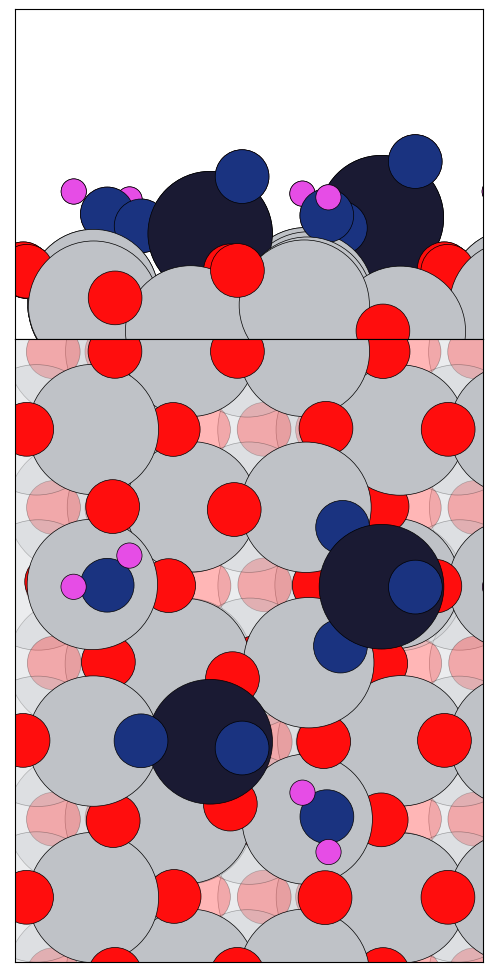
\includegraphics[width=4cm,height=4cm]{V2O5_2H2O_TiO2_101_1by4cell_DFTcsr_Ov_g0.png}  
  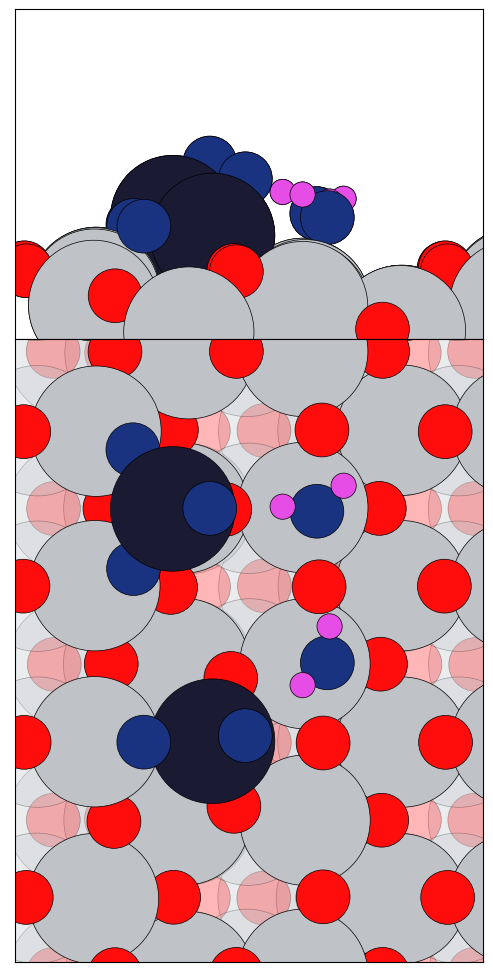
\includegraphics[width=4cm,height=4cm]{V2O5_2H2O_TiO2_101_1by4cell_DFTcsr_Ov_g1.png}  
    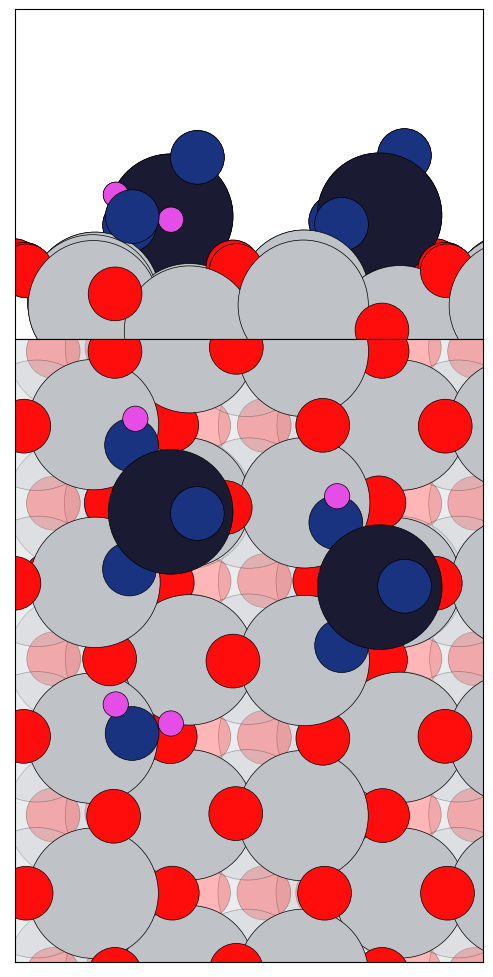
\includegraphics[width=4cm,height=4cm]{V2O5_2H2O_TiO2_101_1by4cell_DFTcsr_Ov_g2.png}  
      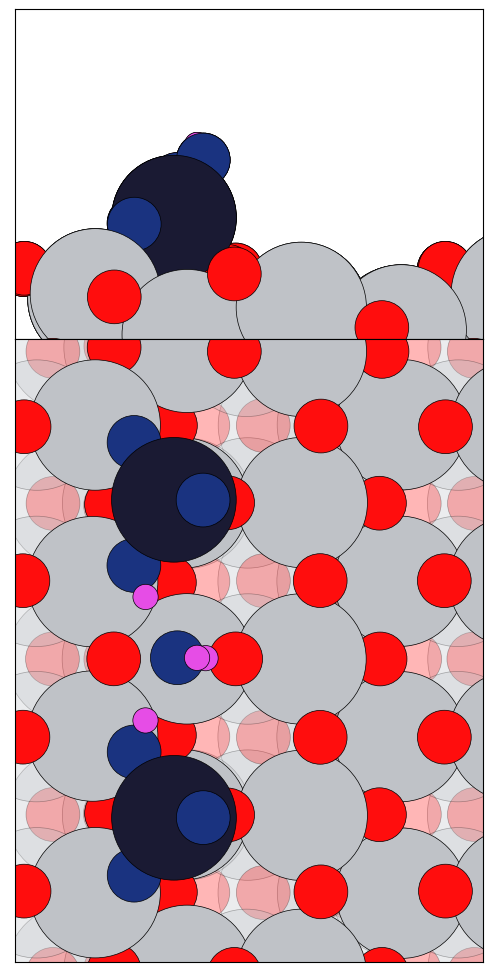
\includegraphics[width=4cm,height=4cm]{V2O5_2H2O_TiO2_101_1by4cell_DFTcsr_Ov_g9.png}  
        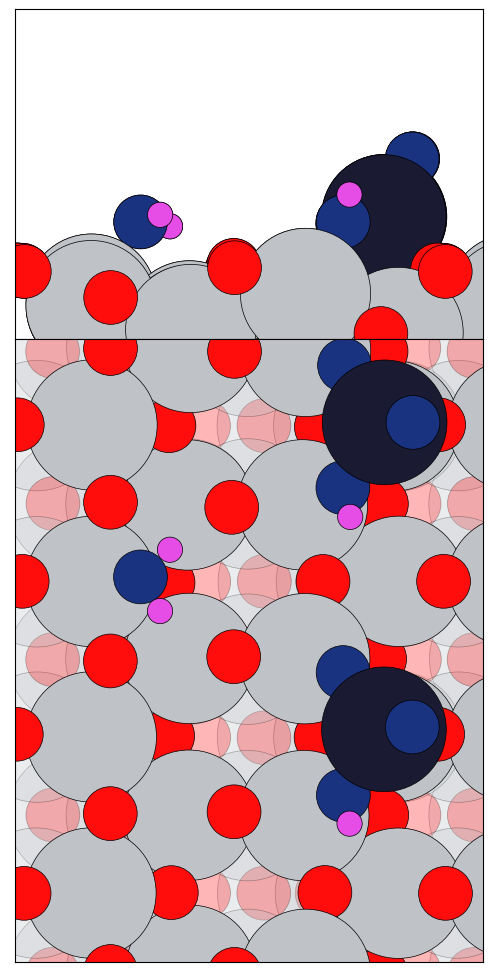
\includegraphics[width=4cm,height=4cm]{V2O5_2H2O_TiO2_101_1by4cell_DFTcsr_Ov_g13.png}  
          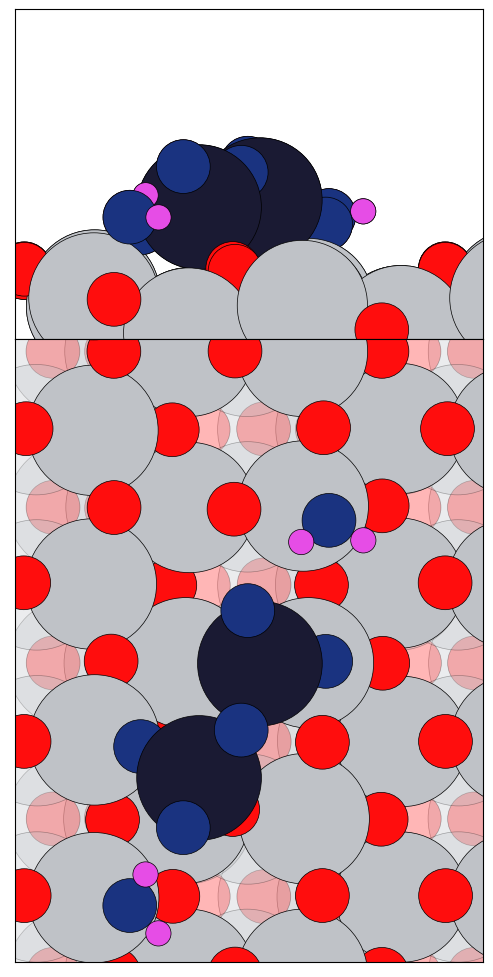
\includegraphics[width=4cm,height=4cm]{V2O5_2H2O_TiO2_101_1by4cell_DFTcsr_Ov_g16.png}  
            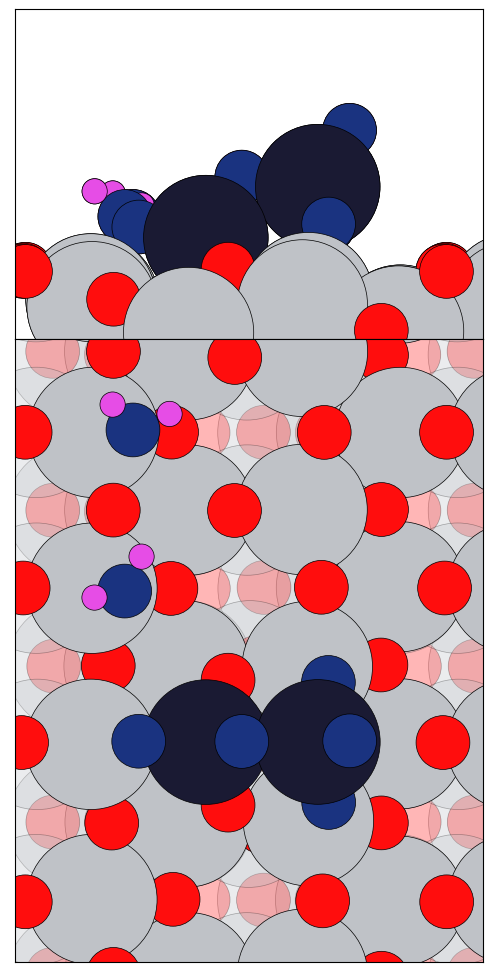
\includegraphics[width=4cm,height=4cm]{V2O5_2H2O_TiO2_101_1by4cell_DFTcsr_Ov_g18.png}  
\caption{Put your caption here}
\label{fig:fig}
\end{figure}


\end{document}


